% This is the Reed College LaTeX thesis template. Most of the work
% for the document class was done by Sam Noble (SN), as well as this
% template. Later comments etc. by Ben Salzberg (BTS). Additional
% restructuring and APA support by Jess Youngberg (JY).
% Your comments and suggestions are more than welcome; please email
% them to cus@reed.edu
%
% See http://web.reed.edu/cis/help/latex.html for help. There are a
% great bunch of help pages there, with notes on
% getting started, bibtex, etc. Go there and read it if you're not
% already familiar with LaTeX.
%
% Any line that starts with a percent symbol is a comment.
% They won't show up in the document, and are useful for notes
% to yourself and explaining commands.
% Commenting also removes a line from the document;
% very handy for troubleshooting problems. -BTS

% As far as I know, this follows the requirements laid out in
% the 2002-2003 Senior Handbook. Ask a librarian to check the
% document before binding. -SN

%%
%% Preamble
%%
% \documentclass{<something>} must begin each LaTeX document
\documentclass[12pt,twoside]{reedthesis}
% Packages are extensions to the basic LaTeX functions. Whatever you
% want to typeset, there is probably a package out there for it.
% Chemistry (chemtex), screenplays, you name it.
% Check out CTAN to see: http://www.ctan.org/
%%
\usepackage{graphicx,latexsym}
\usepackage{amsmath}
\usepackage{amssymb,amsthm}
\usepackage{longtable,booktabs,setspace}
\usepackage{chemarr} %% Useful for one reaction arrow, useless if you're not a chem major
\usepackage[hyphens]{url}
% Added by CII
\usepackage{hyperref}
\usepackage{lmodern}
\usepackage{float}
\floatplacement{figure}{H}
% End of CII addition
\usepackage{rotating}

% Next line commented out by CII
%%% \usepackage{natbib}
% Comment out the natbib line above and uncomment the following two lines to use the new
% biblatex-chicago style, for Chicago A. Also make some changes at the end where the
% bibliography is included.
%\usepackage{biblatex-chicago}
%\bibliography{thesis}


% Added by CII (Thanks, Hadley!)
% Use ref for internal links
\renewcommand{\hyperref}[2][???]{\autoref{#1}}
\def\chapterautorefname{Chapter}
\def\sectionautorefname{Section}
\def\subsectionautorefname{Subsection}
% End of CII addition

% Added by CII
\usepackage{caption}
\captionsetup{width=5in}
% End of CII addition

% \usepackage{times} % other fonts are available like times, bookman, charter, palatino


% To pass between YAML and LaTeX the dollar signs are added by CII
\title{A Game Theoretic Approach to Pokémon Battling}
\author{Samuel D. Olson}
% The month and year that you submit your FINAL draft TO THE LIBRARY (May or December)
\date{May 2017}
\division{Mathematics and Natural Sciences}
\advisor{Prof.~Bray}
%If you have two advisors for some reason, you can use the following
% Uncommented out by CII
\altadvisor{Prof.~Lau}
% End of CII addition

%%% Remember to use the correct department!
\department{Mathematics}
% if you're writing a thesis in an interdisciplinary major,
% uncomment the line below and change the text as appropriate.
% check the Senior Handbook if unsure.
%\thedivisionof{The Established Interdisciplinary Committee for}
% if you want the approval page to say "Approved for the Committee",
% uncomment the next line
%\approvedforthe{Committee}

% Added by CII
%%% Copied from knitr
%% maxwidth is the original width if it's less than linewidth
%% otherwise use linewidth (to make sure the graphics do not exceed the margin)
\makeatletter
\def\maxwidth{ %
  \ifdim\Gin@nat@width>\linewidth
    \linewidth
  \else
    \Gin@nat@width
  \fi
}
\makeatother

\renewcommand{\contentsname}{Table of Contents}
% End of CII addition

\setlength{\parskip}{0pt}

% Added by CII

\providecommand{\tightlist}{%
  \setlength{\itemsep}{0pt}\setlength{\parskip}{0pt}}

\Acknowledgements{
I want to thank a few people.
}

\Dedication{
You can have a dedication here if you wish.
}

\Preface{
This is an example of a thesis setup to use the reed thesis document
class (for LaTeX) and the R bookdown package, in general.
}

\Abstract{
The preface pretty much says it all. \par  Second paragraph of abstract
starts here.
}

% End of CII addition
%%
%% End Preamble
%%
%

\begin{document}

% Everything below added by CII
      \maketitle
  
  \frontmatter % this stuff will be roman-numbered
  \pagestyle{empty} % this removes page numbers from the frontmatter

      \begin{acknowledgements}
      I want to thank a few people.
    \end{acknowledgements}
  
      \begin{preface}
      This is an example of a thesis setup to use the reed thesis document
      class (for LaTeX) and the R bookdown package, in general.
    \end{preface}
  
      \hypersetup{linkcolor=black}
    \setcounter{tocdepth}{2}
    \tableofcontents
  
      \listoftables
  
      \listoffigures
  
      \begin{abstract}
      The preface pretty much says it all. \par  Second paragraph of abstract
      starts here.
    \end{abstract}
  
      \begin{dedication}
      You can have a dedication here if you wish.
    \end{dedication}
  
  \mainmatter % here the regular arabic numbering starts
  \pagestyle{fancyplain} % turns page numbering back on

  \chapter*{Introduction}\label{introduction}
  \addcontentsline{toc}{chapter}{Introduction}
  
  Welcome to the \emph{R Markdown} thesis template. This template is based
  on (and in many places copied directly from) the Reed College LaTeX
  template, but hopefully it will provide a nicer interface for those that
  have never used TeX or LaTeX before. Using \emph{R Markdown} will also
  allow you to easily keep track of your analyses in \textbf{R} chunks of
  code, with the resulting plots and output included as well. The hope is
  this \emph{R Markdown} template gets you in the habit of doing
  reproducible research, which benefits you long-term as a researcher, but
  also will greatly help anyone that is trying to reproduce or build onto
  your results down the road.
  
  Hopefully, you won't have much of a learning period to go through and
  you will reap the benefits of a nicely formatted thesis. The use of
  LaTeX in combination with \emph{Markdown} is more consistent than the
  output of a word processor, much less prone to corruption or crashing,
  and the resulting file is smaller than a Word file. While you may have
  never had problems using Word in the past, your thesis is likely going
  to be about twice as large and complex as anything you've written
  before, taxing Word's capabilities. After working with \emph{Markdown}
  and \textbf{R} together for a few weeks, we are confident this will be
  your reporting style of choice going forward.
  
  \textbf{Why use it?}
  
  \emph{R Markdown} creates a simple and straightforward way to interface
  with the beauty of LaTeX. Packages have been written in \textbf{R} to
  work directly with LaTeX to produce nicely formatting tables and
  paragraphs. In addition to creating a user friendly interface to LaTeX,
  \emph{R Markdown} also allows you to read in your data, to analyze it
  and to visualize it using \textbf{R} functions, and also to provide the
  documentation and commentary on the results of your project. Further, it
  allows for \textbf{R} results to be passed inline to the commentary of
  your results. You'll see more on this later.
  
  \textbf{Who should use it?}
  
  Anyone who needs to use data analysis, math, tables, a lot of figures,
  complex cross-references, or who just cares about the final appearance
  of their document should use \emph{R Markdown}. Of particular use should
  be anyone in the sciences, but the user-friendly nature of
  \emph{Markdown} and its ability to keep track of and easily include
  figures, automatically generate a table of contents, index, references,
  table of figures, etc. should make it of great benefit to nearly anyone
  writing a thesis project.
  
  \chapter{Introduction}\label{introduction-1}
  
  The world of Pokémon began in 1995 with the pair of games Pokémon Red
  and Green. For Westerners, the latter would become known as Pokémon
  Blue. These two games introduced the turn-based battling system that
  became the foundation of the Pokémon games. Numerous other games have
  attempted to copy the Pokémon battling format, but none have been able
  to equal its widespread appeal and dedicated player base. With each
  successive iteration, new items, types, and of course Pokémon are added
  to the Pokémon lexicon. The world of Pokémon has continued to grow and
  evolve into one of the largest video games franchises to date. The most
  recent iterations of Pokémon games, Pokémon Sun and Moon, have continued
  the tradition of adding layers onto an already complex system of
  battling.
  
  Since 2011 the program Pokémon Showdown has offered a `stripped' version
  of Pokémon games. This `stripped' version allows players to exclusively
  battle one another, replicating the most recent iteration of the Pokémon
  games in the process. This has allowed players to hone and test their
  Pokémon battling skills through the years. With well-over 20,000 daily
  registered users and counting, this program has become the go-to program
  to test and practice Pokémon battling strategies in the ultimate pursuit
  of becoming the very best that no one ever was.
  
  To begin formal analysis of Pokémon battling however, the battling
  system must be rigorously detailed for laymen and game theorists alike.
  
  \subsection{A Brief Overview}\label{a-brief-overview}
  
  First, there needs to be a formal model. At its core, Pokémon battling
  takes place exclusively between two players. Each of the two players has
  a team composed of six different Pokémon. Depending on the battle
  format, the team of six Pokémon is either dictated by the player or
  randomly assigned. Regardless of format, each turn each player
  simultaneously makes a decision. The decisions are then executed, with
  priority given first to priority moves and then, if neither player
  decided on a priority move, by a comparative assessment of each
  Pokémon's speed. Once a player's Pokémon loses all of its health, an
  event referred to as fainting, the player must switch into another
  Pokémon. If a player has no other Pokémon to switch into, the battle
  ends. As would be expected, the player whose Pokémon have all fainted
  loses the battle, and the other player wins.
  
  There are a number of parameters and variables to consider beyond those
  already detailed. To begin with, each Pokémon has at most four moves to
  choose from for any turn of a battle. Additionally, whenever a player
  has at least two Pokémon that have not fainted, they have the choice to
  switch into another Pokémon. Doing so counts as the player's action for
  the turn. Thus, players almost always have five different choices to
  make each turn. However, if switches are considered distinct choices,
  the number of potential decisions is at most nine for a given turn.
  Hence, for the purposes of analysis, the supremum of decisions for any
  given turn is nine.
  
  There are a number of other parameters to consider, though these
  parameters are case-specific, i.e.~dependent upon Pokémon, held item,
  Pokémon ability, etc. Such parameters will be further detailed in the
  methodology section, along with further specifications on specific moves
  and Pokémon types.
  
  That being said, Pokémon must be formally denoted as a specific type of
  game in game theoretic terms. With this in mind, it bears noting that
  there are only two outcomes to any battle: One player wins and the other
  loses. Because of this, Pokémon is by definition a zero-sum game.
  However, it is important to note that there are distinct ways that a
  player may win or lose a game. Notably, the same set of decisions made
  by one player over multiple battles may not lead to the same outcome in
  each battle. That is to say, uniqueness of strategies is derived from
  the decisions of both players for any given battle.
  
  A point glossed over previously is the existence of different end games.
  Though the game ends when all of the Pokémon on one team have fainted,
  any player has the choice to forfeit the game any time before this
  occurs. Thus, the two ways to win or lose a battle are either by
  forfeiture or by having all of their Pokémon faint; the latter outcome
  is referred to as a ``normal'' game. Additionally, there is the
  potential for a game to result in a draw. However, draws result in a
  neutral payoff as neither player raises or lowers their ranking after a
  draw.
  
  Within the scope of game theoretic terms, it is vital to note that each
  player is able to see all past decisions made over the course of a
  battle, and that battles span over multiple turns. Speaking to the
  former point, players are able to recall not only their past decisions
  but also those of their opponent, including how much damage was done by
  a specific move during a previous turn. As this information is available
  at any time during the battle, Pokémon battling is a perfect recall
  game. Furthermore as each game is composed of a sequence of turns,
  Pokémon battling is also a sequential game.
  
  The points noted on information allude to a unique trait of Pokémon
  battling that further details the type of game Pokémon battling is: An
  incomplete information game. Though the extent of incompleteness is
  format specific, each player is given limited information about the
  opposing players team at the beginning of the battle. After each turn,
  players are able learn not only the different moves each opposing
  Pokémon has, but also their abilities, held items, and sometimes what
  other Pokémon compose the opposing team. Generally speaking, there is
  almost always new information revealed each turn. The extent to which
  player strategies are revealed from information is an ongoing topic of
  discussion, both here and in current game theory literature. Naturally,
  the analysis of such a topic relies upon at least one apriori
  assumption, namely that player strategies are revealed by their past
  decisions. However, whether player strategies are rational and
  consistent is another matter entirely; nonetheless, at the very least it
  is important to note that incorporating such information into players
  own decision-making complicates analysis and is a central topic in
  analyzing Pokémon battling.
  
  Taken together, Pokémon battling is a special case of a sequential,
  zero-sum two-player game with incomplete information and perfect recall.
  As Pokémon battling lends itself to a discussion of imperfect
  information, it is all the more vital to consider the role of decision
  making in sequential games. A great portion of game theory literature
  has explored such topics, including the revolutionary work of John
  Forbes Nash Jr.
  
  Theoretics aside, there are also notes on the computation side of
  analyzing Pokémon. In this regard, my initial computations and analysis
  focus on the distributions of turn length based on win type, i.e.~the
  length of games played when one player forfeited or had all of their
  Pokémon faint. After distributional computations I categorize moves by
  their type, specifically whether a specific move is damaging,
  non-damaging, or a mix. After categorizing each move individually, I
  then categorize sets of four moves, again using categorizations of
  damaging, non-damaging, or a mix. Using this categorization I gauge the
  effectiveness of specific move sets based on their ability to faint
  Pokémon and by their likelihood to increase a players probability of
  winning.
  
  Overall I hope explore how information gathered turn-by-turn feeds into
  the decision-making process of Pokémon battling. By incorporating
  tenants of behavioral economics and game theory, I hope to rigorously
  analyze and detail phenomena that occur in Pokémon battling. However,
  even more specifically I want to verify the theoretical findings of
  Pokémon battling in a game theoretic framework, specifically the
  existence of one or more mixed Nash equilibrium.
  
  \section{Literature Review}\label{literature-review}
  
  A few points on Pokémon battling are worth noting as they relate Nash's
  literature on game theory mentioned previously. First, each Pokémon
  battle lasts a finite number of turns. Furthermore, each player has
  finitely many choices to make at any given turn. Thus there exists
  finitely many pure strategies for players to choose from each game. Thus
  via application of Nash's Existence Theorem, Pokémon battling has at
  least one Nash equilibrium (Nash 1950).
  
  The question then is to determine what the Nash equilibrium, possibly
  equilibria, is in Pokémon battling. To address this question, it will be
  necessary to consider other theorems and propositions of Nash that
  relate to non-cooperative games. Namely, the goal of analyzing Pokémon
  battling is to determine solutions, strong solutions, and sub-solutions;
  however, it is possible that solutions as defined by Nash do not exist.
  This follows from Nash's note that non-cooperative games do not always
  have a solution; however there do exist sub-solutions (Nash 1951). Thus,
  a central question will be in determining whether Pokémon battling has a
  solution, and if so, if it is unique. Furthermore, it will be important
  to determine what sub-solutions exist, along with how parameterization
  potentially influences such solutions and sub-solutions.
  
  That being said, scant rigorous or academic research has actually been
  conducted within the scope of Pokémon-related topics. The most frequent
  publications focus either on Pokémon as a cultural phenomena or on
  strategy guides for Pokémon games. Importantly, these strategy guides
  have not specifically Pokémon battling strategies, though some have some
  focus on gameplay. However, no Pokémon strategy guides have analyzed
  Pokémon battling by using game theoretic terminology; though that isn't
  to say that there aren't academic publications focusing on Pokémon
  battling.
  
  Typically academic papers focusing on Pokémon battling have focused on
  the use of algorithms to simulate battling strategies and play against
  human players in Pokémon Showdown. One paper gives a rudimentary
  background on Pokémon battling and focuses explicitly on 1v1 battles
  (Gildardo 2013). Since this publication there has been more literature
  however. This literature includes greater nuance, notably by expanding
  the focus of its analysis to teams of six (Ho et al. 2016). Though the
  paper focused on what is currently a previous iteration of Pokémon
  Showdown, the iteration of Pokémon Showdown is fundamentally the same as
  that of the data used here.
  
  Furthermore, relevant documentation of this past iteration of Pokémon
  Showdown is available at its website \url{http://pokemonshowdown.com/}.
  Notably, the website for Pokémon Showdown provides a hub for information
  on Pokémon battling basics and specific battle format descriptions.
  Replays and ladder ranking are available publically, along with links to
  usage statistics and a damage calculator.
  
  As noted previously, game theory vernacular has not entered into
  discussions on Pokémon battling strategies, at least in any formal
  setting. Applying such concepts to the context of Pokémon battling
  offers a formal foundation to discuss strategies and test hypotheses. In
  this regard, there are three main areas of game theory that intersect in
  the analysis of Pokémon battling. These three areas of interest include
  the interpretation of Pokémon battling as a zero sum game, the role of
  incomplete information, and the implications of Pokémon battling as a
  non-cooperative game. These three topics actively influence the
  decision-making process associated with Pokémon battling.
  
  As noted, a central factor involved in the decision making process as it
  relates to game theory is the role of information, specifically how
  players incorporate information revealed each turn into their
  strategies. As information is revealed each turn, including the four
  moves an opposing Pokémon has, its ability, held item, along with what
  other Pokémon are on the opposing team, it is vital for players to
  determine if the information they just received is relevant.
  Furthermore, players need to decide if the information provides any
  insight into their opponent's strategy. Overall, this speaks to Pokémon
  not being a perfect information game. As such, it is not possible to
  apply Zermelo's theorem, though its negation provides insight as to the
  possible existence of a winning strategy (Schwalbe et al. 2001).
  
  An especially interesting addition to the analysis of incomplete
  information in Pokémon battling is the topic and implications of
  asymmetrical information. In this regard, the concepts of sunk costs and
  signaling may enter into the equation. Especially for the Random battle
  format, each player is given minimal information at the onset of the
  game. And while each turn, players both gain information, they may
  receive new information at different rates. The implications of this
  point may provide insight into specific strategies, and is a point of
  future analysis.
  
  This being said, concepts of game theory are not the only relevant ideas
  for analyzing Pokémon battling. In this vein, exploring whether a player
  will switch Pokémon will necessarily invoke ideas from game theory and
  behavioral economics. One specific concept engrained in behavioral
  economics that relates to Pokémon battling is the idea of ``keeping
  doors open''. In Chapter 6 of Ariel's work Predictably Irrational,
  results indicates that players prefer to keep options available even if
  doing so incurs costs and/or reduces their payoff. In the context of
  Pokémon battling, players may decide to preemptively switch Pokémon in
  the hopes of having that Pokémon later in the battle. However, whether
  this adversely influences the player is yet another subject of inquiry.
  
  A an ending point of interest, taking into account opposing players'
  strategies as deduced from revealed information rubs against issues
  related level-K thinking. To elaborate further, knowing that a player is
  likely to repeat the same decision made the previous turn, players may
  be able optimize their decision by presuposing what decision their
  opponent is going to make. However, if the opposing player decides to
  incorporate that very assumption into their own decision, they may
  arrive at a vastly different outcome than would be expected. Furthermore
  this outcome may even be suboptimal for both players. That being said,
  the inclusion of level-k thinking is closely aligned to recent
  behavioral game theory literature. A central finding of this literature
  has emphasized the role of iterated reasoning, which essentializes
  player adaptation to other players' decision making (Wunder et al.
  2011). Notably this will be a point to consider and incorporate into the
  analysis of Pokémon battling in a game theoretic framework.
  
  \section{References}\label{references}
  
  \begin{itemize}
  \tightlist
  \item
    Ariely, D. (2009). Predictably irrational: The hidden forces that
    shape our decisions. New York, NY: Harper. Chapter 8: Keeping Doors
    Open (pp.~139-154).
  \item
    Schwalbe, U., \& Walker, P. (2001). Zermelo and the Early History of
    Game Theory. Games and Economic Behavior, 34(1), 123-137.
    \url{doi:10.1006/game.2000.0794}
  \item
    Smogon University (n.d.). Retrieved October 31, 2016, from
    \url{http://www.smogon.com/}
  \item
    Pokémon Showdown! battle simulator (n.d.). Retrieved October 31, 2016,
    from \url{http://pokemonshowdown.com/}
  \item
    Pokémon Showdown Github Master Repository (2016).
    Zarel/Pokemon-Showdown. Retrieved October 31, 2016, from
    \url{https://github.com/Zarel/Pokemon-Showdown/tree/master/data}
  \item
    Wunder, M., Kaisers, M., Yaros, J., Littman, M., (May, 2011) Using
    Iterated Reasoning to Predict Opponent Strategies. Proc. of 10th Int.
    Conf. on Autonomous Agents and Multiagent Systems (AAMAS 2011), Tumer,
    Yolum, Sonenberg and Stone (eds.), 593-600.
  \item
    Ho, H., Ramesh, V. (2016) Percymon: A Pokemon Showdown Artifical
    Intelligence. Retrieved October 31, 2016, from:
    \url{http://robots.stanford.edu/cs221/2016/restricted/projects/vramesh2/final.pdf}
  \item
    Sanchez-Ante, Gildardo (Dec., 2013) Sistemas Inteligentes: Reportes
    Finales Ago-Dic 2013. Retrieved October 31, 2016, from:
    \url{https://www.researchgate.net/profile/Gildardo_Sanchez-Ante/publication/259343975_Sistemas_Inteligentes_Reportes_Finales_Ago-Dic_2013/links/0c96052b1d0b582e95000000.pdf\#page=140}
  \item
    Pokémon Company International (Nov. 21, 2014) Pokémon Omega Ruby \&
    Pokémon Alpha Sapphire: The Official Hoenn Region Strategy Guide.
  \item
    Nash, J. F., Jr. (1950, January 15). Equilibrium Points in n-Person
    Games. Proceedings of the National Academy of Sciences of the United
    States of America, 36(1), 48-49. Retrieved November 29, 2016, from
    \url{http://www.sscnet.ucla.edu/polisci/faculty/chwe/austen/nash1950.pdf}
  \item
    Nash, J. F., Jr. (1951, September). Non-Cooperative Games. The Annals
    of Mathematics, Second Series, 54(2), 286-295. Retrieved November 29,
    2016, from
    \url{http://lcm.csa.iisc.ernet.in/gametheory/Classics/NCG.pdf}
  \end{itemize}
  
  \section{Methodology}\label{methodology}
  
  The data used is a compilation of battle logs from the Pokémon Showdown
  servers. Each battle log is stored as a separate .json file. The data
  spans across the year 2015, composed of four different months of data.
  The four months are March, June, September, and December. There are no
  lapses in data, i.e.~each day of each month has numerous battle logs to
  account for. No dramatic overhaul was done to the Pokémon battling
  format at this time, though some minor adjustments were made.
  Furthermore only ranked games are included in the dataset, indicating
  that each player stands to gain or lose from the battle.
  
  Specific usage statistics are found in a subsidiary website, found at
  \url{http://sweepercalc.com/stats/}. The usage statistics track the
  frequency of use for specific Pokémon, items, abilities, and a host of
  other relevant variables for Pokémon battling.
  
  A number of links redirect users to the host site of this game: Smogon
  University. The host site can be found at \url{http://www.smogon.com/}.
  This website offers a wide variety of resources, similar to those found
  at the Pokémon Showdown website. Most importantly the Smogon forums are
  a prominent site for discussion of Pokémon battling strategies.
  
  \subsection{Pokémon Battling Basics}\label{pokemon-battling-basics}
  
  The Pokémon battle starts with Pokémon being sent out. For the purposes
  of the data used, one Pokémon is sent out for each opponent, totalling
  two Pokémon being out at any given time. Following this, each Pokémon
  has 4 moves to choose from, along with the option to switch to a
  different Pokémon (when applicable). After both players make a decision,
  the moves are weighted for priority and speed to determine the order of
  play. If both players decide not to switch one Pokémon will attack the
  other, after which the next Pokémon will do the same if it has not
  fainted. After each move has been executed the turn ends and the process
  is repeated. When one of the Pokémon faints, the player whose Pokémon
  fainted will be prompted to select another Pokémon from the bench. The
  first player to lose all of their Pokémon loses the battle.
  
  \subsubsection{Battle Formats}\label{battle-formats}
  
  The data used for this study include two different Pokémon battling
  formats. The two formats are known as Over Used and Random Battles,
  abbreviated as OU and Randbats respectively. Both formats have teams of
  six Pokémon and only allow one Pokémon to be out at any given time.
  While both battle formats are subsets of what are known as single
  battles, each has their own unique spin on the Pokémon battling format.
  
  Random Battles are the most frequently played format. Neither player
  gets to decide on their initial Pokémon nor do they have any input on
  the composition of the team. The format uses an algorithm to determine
  team compositions. However it is important to note that there are
  restrictions to the Randbats format that center around team composition
  and move composition for specific Pokémon.
  
  The Over Used battle format includes team composition. By including team
  composition, players are able to decide what Pokémon to include on their
  team, the moves of each Pokémon, and other factors such as held items
  and abilities. Further restrictions to the OU format include banning
  specific Pokémon. The restricted Pokémon are included in the ``Uber''
  tier along with the Pokémon Mega-Rayquaza. Additionally certain
  ``hidden'' abilities are locked for Pokémon.
  
  \subsection{Pokémon Attributes}\label{pokemon-attributes}
  
  Generally, there are a number of factors that are specific to each
  Pokémon. Some of these factors are considered static, meaning that they
  do not change over the course of the battle. These types of factors are
  noted as ``Fixed'' Attributes. However there are some factors that are
  generally regarded as Fixed Attributes but are affected by certain
  moves, at least when the Pokémon is sent out. These types of factors are
  a distinct subcategory of ``Variable Attributes'', and will be outlined
  further. Additionally there are attributes that are inherently
  influenced throughout the course of the battle. These are noted as
  ``Variable Attributes''. The terminology is largely taken from the Ho et
  al. paper for ease of translation.
  
  \subsubsection{Pokémon Types}\label{pokemon-types}
  
  The type(s) of each Pokémon influence not only the potential weaknesses
  of each Pokémon, but also influence the amount of damage certain
  type-specific moves are able to do. Each Pokémon has at least one and at
  most two types. If a Pokémon uses a damaging move whose type corresponds
  to type of the Pokémon that used it, that Pokémon gets a same type
  attack bonus, abbreviated as a ``stab'' bonus. This causes the move to
  do 50\% more damage, potentially 100\% if the Pokémon also has the
  ability Adaptability.
  
  \subsubsection{Pokémon Fixed Attributes}\label{pokemon-fixed-attributes}
  
  Fixed attributes include the type(s) of the Pokémon, the four moves the
  Pokémon has learned, the one item the Pokémon holds, the Pokémon's one
  selected ability, the level of the Pokémon, and the Pokémon's baseline
  stats. The latter factor is divided into six categories. These
  categories include (baseline) Health, Attack, Special Attack, Defense,
  Special Defense, and Speed. There is further nuance with the inclusion
  of Pokémon natures and Individual Values, or IVs. These factors
  influence the base stats of each Pokémon. However due to the sheer
  number of trivial combinations of IV spreads and nature choices, these
  two factors will not be a pivotal aspect of framework used.
  
  \subsubsection{Pokémon Variable
  Attributes}\label{pokemon-variable-attributes}
  
  Variable Attributes include the current health of the Pokémon, the
  status of the Pokémon, the volatile status of the Pokémon, boost data of
  the Pokémon, and whether the Pokémon in question is currently active.
  
  \subsection{Game Theory Methodology}\label{game-theory-methodology}
  
  Let the index of Player 1 and 2's Pokémon be denoted by i and j
  respectively. Let the set of Player 1's Pokémon be given as follows:
  \[A=\{A_1,A_2,A_3,A_4,A_5,A_6\}\] Similarly let the set of player 2's
  Pokémon be given by: \[B=\{B_1,B_2,B_3,B_4,B_5,B_6\}\] Furthermore let N
  denote the number of turns a given Pokémon battle lasts. Let the
  cumulative total of damage done to Player 1's ith Pokémon be denoted:
  \(\sum_{t=0}^{N} d_{A_i,t}\). It follows that the damage done to Player
  1's ith Pokémon on turn t is given by: \(d_{A_i,t}\) Similarly tet the
  cumulative total of damage done to Player 2's jth Pokémon is given by:
  \(\sum_{t=0}^{N} d_{B_j,t}\); additionally, the damage done to Player
  2's jth Pokémon on turn t is given by: \(d_{B_j,t}\)
  
  Let the payoff function of Player 1 and Player 2 be respectively denoted
  by \(P_1 and P_2\). Note that neither player is able to revive a fainted
  Pokémon during a battle. Thus, the amount of damage done to an
  opponent's Pokémon directly corresponds to the payoff they receive
  during a given turn. Furthermore, players are able to utilize moves that
  heal their Pokémon during the turn. Thus, the payoff function must
  include not only the current health of the opposing Pokémon, but also
  the amount of damage done to the opponent's Pokémon and the amount of
  health the opponent's Pokémon heals during the turn. Additionally, it is
  important to incorporate the current health of the opponent's Pokémon at
  the beginning of the turn. This is to account for potential healing and
  damage that may result at the end of each turn.
  
  Let the current health of Player 2's jth Pokémon on turn t be given
  by:\(H_{B_{j,t}}\). Furthermore, let the amount of damage done to Player
  2's jth Pokémon on turn t be given by: \(d_{B_{j,t}}\). Finally let
  \(h_{B{j,t}}\) denote the amount of health regained by Player 2's jth
  Pokémon on turn t. We may write the payoff function at turn t as a
  function of three variables. However, it is important to note that while
  damage is independent of current health and healing done on turn t, the
  amount of healing done to an opponent's Pokémon is contrained by it's
  health at the beginning of turn t.
  
  Thus we may write \(P_1\) as a function of \(H_{B_{j,t}}\),
  \(d_{B_{j,t}}\), \(h_{B{j,t}}\). Next, let an opponent's fainted Pokémon
  corresponds to a payoff of 1. As each player has six Pokémon,
  max(\(P_1\))=6. This payoff corresponds to Player 1 fainting all of
  Player 2's Pokémon.
  
  Now we need to create an equation to model the payoff of Player 1 at
  turn t. To do so, we need to construct a piecewise function that
  corresponds to the values given previously. To begin with, we note that
  if Player 1's damage to the opposing Pokémon is greater than that
  opposing Pokémon's health at the beginning of the turn, that Pokémon
  faints. Intuitively, this means that the payoff from fainting an
  opponent's Pokémon is the same for Player 1 regardless of whether they
  exceeded the amount of damage needed to faint the opponents Pokémon.
  With this in mind, let \(n_1\) denote the number of Pokémon Player 1 has
  knocked out. We may then write the payoff function for Player 1 after
  turn t as follows: \[P(H,h,d)_{1,t} = \left\{
          \begin{array}{ll}
              n_1 +1  &\quad if (\sum_{t=0}^{N} d_{B_i,t} - h_{B{j,t}}) > H_{B_{j,t}}\\
              (n_1 + \sum_{t=0}^{N} (d_{A_i,t} - h_{B{j,t}}))/H_{B_{j,t}}& \quad otherwise
          \end{array}
      \right.
  \]
  
  We now have an equation to model the payoff function of Player 1 at any
  turn of a Pokémon battle. Let \(n_2\) denote the number of Pokémon
  Player 2 has knocked out. Thus, we may similarly construct a piecewise
  function for Player 2's payoff function at turn t as:
  \[P(H,h,d)_{2,t} = \left\{
          \begin{array}{ll}
              n_2 + 1  &\quad if (\sum_{t=0}^{N} d_{A_i,t} - h_{A{j,t}}) > H_{B_{j,t}}\\
              (n_2 + \sum_{t=0}^{N} (d_{A_i,t} - h_{A{j,t}}))/H_{A_{j,t}}& \quad otherwise
          \end{array}
      \right.
  \]
  
  We may now assemble the ordered pairs corresponding to each combination
  of Player 1 and Player 2's possible decisions for any given turn.
  However, before doing so, it is important to note that the three
  functions corresponding to Pokémon health, damage, and healing are left
  for further detailing. Before going on to the normal form version of
  Pokémon battling, these functions will be given further detail.
  
  \subsubsection{Creating the Damage
  Function}\label{creating-the-damage-function}
  
  \subsubsection{Normal Form Version of Pokémon
  Battling}\label{normal-form-version-of-pokemon-battling}
  
  \section{End thesis Chapter 1}\label{end-thesis-chapter-1}
  
  \chapter{MARKDOWN TEMPLATE}\label{markdown-template}
  
  \begin{Shaded}
  \begin{Highlighting}[]
  \KeywordTok{summary}\NormalTok{(cars)}
  \end{Highlighting}
  \end{Shaded}
  
  \begin{verbatim}
       speed           dist       
   Min.   : 4.0   Min.   :  2.00  
   1st Qu.:12.0   1st Qu.: 26.00  
   Median :15.0   Median : 36.00  
   Mean   :15.4   Mean   : 42.98  
   3rd Qu.:19.0   3rd Qu.: 56.00  
   Max.   :25.0   Max.   :120.00  
  \end{verbatim}
  
  \section{Inline code}\label{inline-code}
  
  If you'd like to put the results of your analysis directly into your
  discussion, add inline code like this:
  
  \begin{quote}
  The \texttt{cos} of \(2 \pi\) is 1.
  \end{quote}
  
  Another example would be the direct calculation of the standard
  deviation:
  
  \begin{quote}
  The standard deviation of \texttt{speed} in \texttt{cars} is 5.2876444.
  \end{quote}
  
  One last neat feature is the use of the \texttt{ifelse} conditional
  statement which can be used to output text depending on the result of an
  \textbf{R} calculation:
  
  \begin{quote}
  The standard deviation is less than 6.
  \end{quote}
  
  Note the use of \texttt{\textgreater{}} here, which signifies a
  quotation environment that will be indented.
  
  As you see with \texttt{\$2\ \textbackslash{}pi\$} above, mathematics
  can be added by surrounding the mathematical text with dollar signs.
  More examples of this are in \protect\hyperlink{math-sci}{Mathematics
  and Science} if you uncomment the code in
  \protect\hyperlink{math}{Math}.
  
  \section{Including plots}\label{including-plots}
  
  You can also embed plots. For example, here is a way to use the base
  \textbf{R} graphics package to produce a plot using the built-in
  \texttt{pressure} dataset:
  
  \begin{center}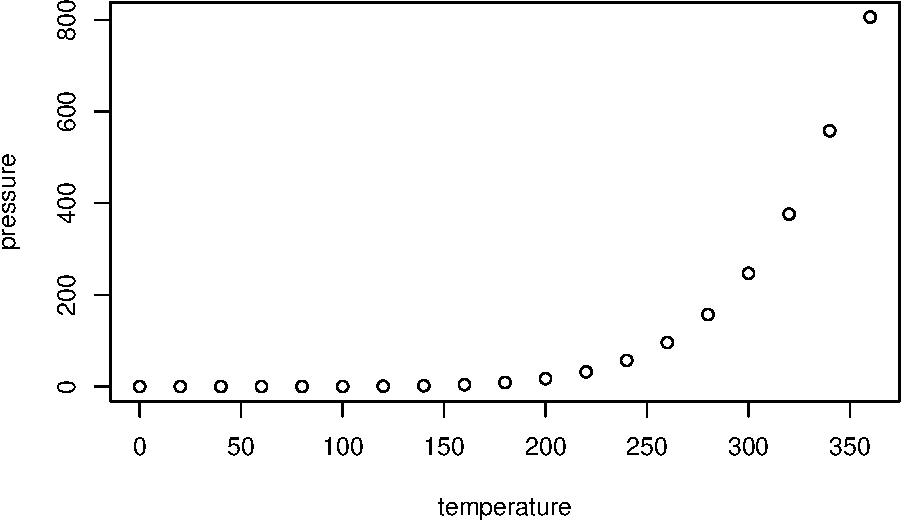
\includegraphics{thesis_files/figure-latex/pressure-1} \end{center}
  
  Note that the \texttt{echo=FALSE} parameter was added to the code chunk
  to prevent printing of the \textbf{R} code that generated the plot.
  There are plenty of other ways to add chunk options. More information is
  available at \url{http://yihui.name/knitr/options/}.
  
  Another useful chunk option is the setting of \texttt{cache=TRUE} as you
  see here. If document rendering becomes time consuming due to long
  computations or plots that are expensive to generate you can use knitr
  caching to improve performance. Later in this file, you'll see a way to
  reference plots created in \textbf{R} or external figures.
  
  \hypertarget{loading-and-exploring-data}{\section{Loading and exploring
  data}\label{loading-and-exploring-data}}
  
  Included in this template is a file called \texttt{flights.csv}. This
  file includes a subset of the larger dataset of information about all
  flights that departed from Seattle and Portland in 2014. More
  information about this dataset and its \textbf{R} package is available
  at \url{http://github.com/ismayc/pnwflights14}. This subset includes
  only Portland flights and only rows that were complete with no missing
  values. Merges were also done with the \texttt{airports} and
  \texttt{airlines} data sets in the \texttt{pnwflights14} package to get
  more descriptive airport and airline names.
  
  We can load in this data set using the following command:
  
  \begin{Shaded}
  \begin{Highlighting}[]
  \NormalTok{flights <-}\StringTok{ }\KeywordTok{read.csv}\NormalTok{(}\StringTok{"data/flights.csv"}\NormalTok{)}
  \end{Highlighting}
  \end{Shaded}
  
  The data is now stored in the data frame called \texttt{flights} in
  \textbf{R}. To get a better feel for the variables included in this
  dataset we can use a variety of functions. Here we can see the
  dimensions (rows by columns) and also the names of the columns.
  
  \begin{Shaded}
  \begin{Highlighting}[]
  \KeywordTok{dim}\NormalTok{(flights)}
  \end{Highlighting}
  \end{Shaded}
  
  \begin{verbatim}
  [1] 52808    16
  \end{verbatim}
  
  \begin{Shaded}
  \begin{Highlighting}[]
  \KeywordTok{names}\NormalTok{(flights)}
  \end{Highlighting}
  \end{Shaded}
  
  \begin{verbatim}
   [1] "month"        "day"          "dep_time"     "dep_delay"   
   [5] "arr_time"     "arr_delay"    "carrier"      "tailnum"     
   [9] "flight"       "dest"         "air_time"     "distance"    
  [13] "hour"         "minute"       "carrier_name" "dest_name"   
  \end{verbatim}
  
  Another good idea is to take a look at the dataset in table form. With
  this dataset having more than 50,000 rows, we won't explicitly show the
  results of the command here. I recommend you enter the command into the
  Console \textbf{\emph{after}} you have run the \textbf{R} chunks above
  to load the data into \textbf{R}.
  
  \begin{Shaded}
  \begin{Highlighting}[]
  \KeywordTok{View}\NormalTok{(flights)}
  \end{Highlighting}
  \end{Shaded}
  
  While not required, it is highly recommended you use the \texttt{dplyr}
  package to manipulate and summarize your data set as needed. It uses a
  syntax that is easy to understand using chaining operations. Below I've
  created a few examples of using \texttt{dplyr} to get information about
  the Portland flights in 2014. You will also see the use of the
  \texttt{ggplot2} package, which produces beautiful, high-quality
  academic visuals.
  
  We begin by checking to ensure that needed packages are installed and
  then we load them into our current working environment:
  
  \begin{Shaded}
  \begin{Highlighting}[]
  \CommentTok{# List of packages required for this analysis}
  \NormalTok{pkg <-}\StringTok{ }\KeywordTok{c}\NormalTok{(}\StringTok{"dplyr"}\NormalTok{, }\StringTok{"ggplot2"}\NormalTok{, }\StringTok{"knitr"}\NormalTok{, }\StringTok{"bookdown"}\NormalTok{, }\StringTok{"devtools"}\NormalTok{)}
  \CommentTok{# Check if packages are not installed and assign the}
  \CommentTok{# names of the packages not installed to the variable new.pkg}
  \NormalTok{new.pkg <-}\StringTok{ }\NormalTok{pkg[!(pkg %in%}\StringTok{ }\KeywordTok{installed.packages}\NormalTok{())]}
  \CommentTok{# If there are any packages in the list that aren't installed,}
  \CommentTok{# install them}
  \NormalTok{if (}\KeywordTok{length}\NormalTok{(new.pkg))}
    \KeywordTok{install.packages}\NormalTok{(new.pkg, }\DataTypeTok{repos =} \StringTok{"http://cran.rstudio.com"}\NormalTok{)}
  \CommentTok{# Load packages (thesisdown will load all of the packages as well)}
  \KeywordTok{library}\NormalTok{(thesisdown)}
  \end{Highlighting}
  \end{Shaded}
  
  \clearpage
  
  The example we show here does the following:
  
  \begin{itemize}
  \item
    Selects only the \texttt{carrier\_name} and \texttt{arr\_delay} from
    the \texttt{flights} dataset and then assigns this subset to a new
    variable called \texttt{flights2}.
  \item
    Using \texttt{flights2}, we determine the largest arrival delay for
    each of the carriers.
  \end{itemize}
  
  \begin{Shaded}
  \begin{Highlighting}[]
  \NormalTok{flights2 <-}\StringTok{ }\NormalTok{flights %>%}\StringTok{ }
  \StringTok{  }\KeywordTok{select}\NormalTok{(carrier_name, arr_delay)}
  \NormalTok{max_delays <-}\StringTok{ }\NormalTok{flights2 %>%}\StringTok{ }
  \StringTok{  }\KeywordTok{group_by}\NormalTok{(carrier_name) %>%}
  \StringTok{  }\KeywordTok{summarize}\NormalTok{(}\DataTypeTok{max_arr_delay =} \KeywordTok{max}\NormalTok{(arr_delay, }\DataTypeTok{na.rm =} \OtherTok{TRUE}\NormalTok{))}
  \end{Highlighting}
  \end{Shaded}
  
  A useful function in the \texttt{knitr} package for making nice tables
  in \emph{R Markdown} is called \texttt{kable}. It is much easier to use
  than manually entering values into a table by copying and pasting values
  into Excel or LaTeX. This again goes to show how nice reproducible
  documents can be! (Note the use of \texttt{results="asis"}, which will
  produce the table instead of the code to create the table.) The
  \texttt{caption.short} argument is used to include a shorter title to
  appear in the List of Tables.
  
  \begin{Shaded}
  \begin{Highlighting}[]
  \KeywordTok{kable}\NormalTok{(max_delays, }
        \DataTypeTok{col.names =} \KeywordTok{c}\NormalTok{(}\StringTok{"Airline"}\NormalTok{, }\StringTok{"Max Arrival Delay"}\NormalTok{),}
        \DataTypeTok{caption =} \StringTok{"Maximum Delays by Airline"}\NormalTok{,}
        \DataTypeTok{caption.short =} \StringTok{"Max Delays by Airline"}\NormalTok{,}
        \DataTypeTok{longtable =} \OtherTok{TRUE}\NormalTok{,}
        \DataTypeTok{booktabs =} \OtherTok{TRUE}\NormalTok{)}
  \end{Highlighting}
  \end{Shaded}
  
  \begin{longtable}[t]{lr}
  \caption[Max Delays by Airline]{\label{tab:maxdelays}Maximum Delays by Airline}\\
  \toprule
  Airline & Max Arrival Delay\\
  \midrule
  Alaska Airlines Inc. & 338\\
  American Airlines Inc. & 1539\\
  Delta Air Lines Inc. & 651\\
  Frontier Airlines Inc. & 575\\
  Hawaiian Airlines Inc. & 407\\
  \addlinespace
  JetBlue Airways & 273\\
  SkyWest Airlines Inc. & 421\\
  Southwest Airlines Co. & 694\\
  United Air Lines Inc. & 472\\
  US Airways Inc. & 347\\
  Virgin America & 366\\
  \bottomrule
  \end{longtable}
  
  The last two options make the table a little easier-to-read.
  
  We can further look into the properties of the largest value here for
  American Airlines Inc. To do so, we can isolate the row corresponding to
  the arrival delay of 1539 minutes for American in our original
  \texttt{flights} dataset.
  
  \begin{Shaded}
  \begin{Highlighting}[]
  \NormalTok{flights %>%}\StringTok{ }\KeywordTok{filter}\NormalTok{(arr_delay ==}\StringTok{ }\DecValTok{1539}\NormalTok{, }
                    \NormalTok{carrier_name ==}\StringTok{ "American Airlines Inc."}\NormalTok{) %>%}
  \StringTok{  }\KeywordTok{select}\NormalTok{(-}\KeywordTok{c}\NormalTok{(month, day, carrier, dest_name, hour, }
              \NormalTok{minute, carrier_name, arr_delay))}
  \end{Highlighting}
  \end{Shaded}
  
  \begin{verbatim}
    dep_time dep_delay arr_time tailnum flight dest air_time distance
  1     1403      1553     1934  N595AA   1568  DFW      182     1616
  \end{verbatim}
  
  We see that the flight occurred on March 3rd and departed a little after
  2 PM on its way to Dallas/Fort Worth. Lastly, we show how we can
  visualize the arrival delay of all departing flights from Portland on
  March 3rd against time of departure.
  
  \begin{Shaded}
  \begin{Highlighting}[]
  \NormalTok{flights %>%}\StringTok{ }\KeywordTok{filter}\NormalTok{(month ==}\StringTok{ }\DecValTok{3}\NormalTok{, day ==}\StringTok{ }\DecValTok{3}\NormalTok{) %>%}
  \StringTok{  }\KeywordTok{ggplot}\NormalTok{(}\KeywordTok{aes}\NormalTok{(}\DataTypeTok{x =} \NormalTok{dep_time, }\DataTypeTok{y =} \NormalTok{arr_delay)) +}\StringTok{ }\KeywordTok{geom_point}\NormalTok{()}
  \end{Highlighting}
  \end{Shaded}
  
  \begin{center}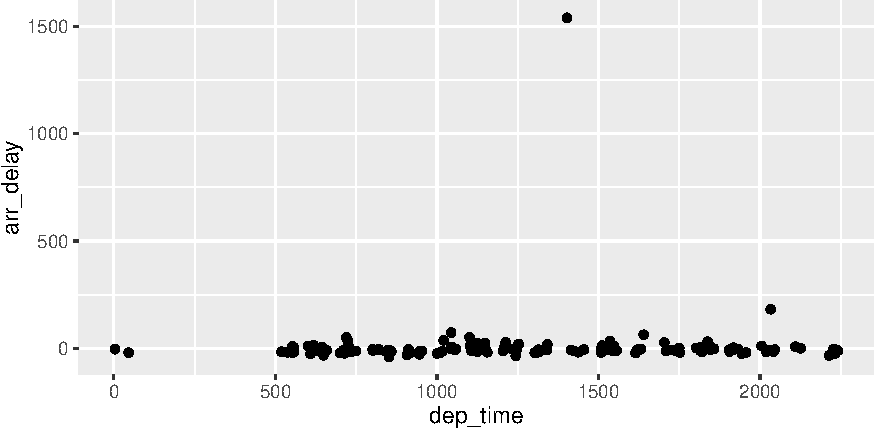
\includegraphics{thesis_files/figure-latex/march3plot-1} \end{center}
  
  \section{Additional resources}\label{additional-resources}
  
  \begin{itemize}
  \item
    \emph{Markdown} Cheatsheet -
    \url{https://github.com/adam-p/markdown-here/wiki/Markdown-Cheatsheet}
  \item
    \emph{R Markdown} Reference Guide -
    \url{https://www.rstudio.com/wp-content/uploads/2015/03/rmarkdown-reference.pdf}
  \item
    Introduction to \texttt{dplyr} -
    \url{https://cran.rstudio.com/web/packages/dplyr/vignettes/introduction.html}
  \item
    \texttt{ggplot2} Documentation -
    \url{http://docs.ggplot2.org/current/}
  \end{itemize}
  
  \hypertarget{math-sci}{\chapter{Mathematics and
  Science}\label{math-sci}}
  
  \hypertarget{math}{\section{Math}\label{math}}
  
  \TeX~is the best way to typeset mathematics. Donald Knuth designed
  \TeX~when he got frustrated at how long it was taking the typesetters to
  finish his book, which contained a lot of mathematics. One nice feature
  of \emph{R Markdown} is its ability to read LaTeX code directly.
  
  If you are doing a thesis that will involve lots of math, you will want
  to read the following section which has been commented out. If you're
  not going to use math, skip over or delete this next commented section.
  
  \section{Chemistry 101: Symbols}\label{chemistry-101-symbols}
  
  Chemical formulas will look best if they are not italicized. Get around
  math mode's automatic italicizing in LaTeX by using the argument
  \texttt{\$\textbackslash{}mathrm\{formula\ here\}\$}, with your formula
  inside the curly brackets. (Notice the use of the backticks here which
  enclose text that acts as code.)
  
  So, \(\mathrm{Fe_2^{2+}Cr_2O_4}\) is written
  \texttt{\$\textbackslash{}mathrm\{Fe\_2\^{}\{2+\}Cr\_2O\_4\}\$}.
  
  \noindent Exponent or Superscript: \(\mathrm{O^-}\)
  
  \noindent Subscript: \(\mathrm{CH_4}\)
  
  To stack numbers or letters as in \(\mathrm{Fe_2^{2+}}\), the subscript
  is defined first, and then the superscript is defined.
  
  \noindent Bullet: CuCl \(\bullet\) \(\mathrm{7H_{2}O}\)
  
  \noindent Delta: \(\Delta\)
  
  \noindent Reaction Arrows: \(\longrightarrow\) or
  \(\xrightarrow{solution}\)
  
  \noindent Resonance Arrows: \(\leftrightarrow\)
  
  \noindent Reversible Reaction Arrows: \(\rightleftharpoons\)
  
  \subsection{Typesetting reactions}\label{typesetting-reactions}
  
  You may wish to put your reaction in an equation environment, which
  means that LaTeX will place the reaction where it fits and will number
  the equations for you.
  
  \begin{equation}
    \mathrm{C_6H_{12}O_6  + 6O_2} \longrightarrow \mathrm{6CO_2 + 6H_2O}
    \label{eq:reaction}
  \end{equation}
  
  We can reference this combustion of glucose reaction via Equation
  \ref{eq:reaction}.
  
  \subsection{Other examples of
  reactions}\label{other-examples-of-reactions}
  
  \(\mathrm{NH_4Cl_{(s)}}\) \(\rightleftharpoons\)
  \(\mathrm{NH_{3(g)}+HCl_{(g)}}\)
  
  \noindent \(\mathrm{MeCH_2Br + Mg}\) \(\xrightarrow[below]{above}\)
  \(\mathrm{MeCH_2\bullet Mg \bullet Br}\)
  
  \section{Physics}\label{physics}
  
  Many of the symbols you will need can be found on the math page
  \url{http://web.reed.edu/cis/help/latex/math.html} and the Comprehensive
  LaTeX Symbol Guide
  (\url{http://mirror.utexas.edu/ctan/info/symbols/comprehensive/symbols-letter.pdf}).
  
  \section{Biology}\label{biology}
  
  You will probably find the resources at
  \url{http://www.lecb.ncifcrf.gov/~toms/latex.html} helpful, particularly
  the links to bsts for various journals. You may also be interested in
  TeXShade for nucleotide typesetting
  (\url{http://homepages.uni-tuebingen.de/beitz/txe.html}). Be sure to
  read the proceeding chapter on graphics and tables.
  
  \chapter{Tables, Graphics, References, and Labels}\label{ref-labels}
  
  \section{Tables}\label{tables}
  
  In addition to the tables that can be automatically generated from a
  data frame in \textbf{R} that you saw in {[}R Markdown Basics{]} using
  the \texttt{kable} function, you can also create tables using
  \emph{pandoc}. (More information is available at
  \url{http://pandoc.org/README.html\#tables}.) This might be useful if
  you don't have values specifically stored in \textbf{R}, but you'd like
  to display them in table form. Below is an example. Pay careful
  attention to the alignment in the table and hyphens to create the rows
  and columns.
  
  \begin{longtable}[c]{@{}ccc@{}}
  \caption{\label{tab:inher} Correlation of Inheritance Factors for Parents
  and Child}\tabularnewline
  \toprule
  \begin{minipage}[b]{0.29\columnwidth}\centering\strut
  Factors
  \strut\end{minipage} &
  \begin{minipage}[b]{0.47\columnwidth}\centering\strut
  Correlation between Parents \& Child
  \strut\end{minipage} &
  \begin{minipage}[b]{0.16\columnwidth}\centering\strut
  Inherited
  \strut\end{minipage}\tabularnewline
  \midrule
  \endfirsthead
  \toprule
  \begin{minipage}[b]{0.29\columnwidth}\centering\strut
  Factors
  \strut\end{minipage} &
  \begin{minipage}[b]{0.47\columnwidth}\centering\strut
  Correlation between Parents \& Child
  \strut\end{minipage} &
  \begin{minipage}[b]{0.16\columnwidth}\centering\strut
  Inherited
  \strut\end{minipage}\tabularnewline
  \midrule
  \endhead
  \begin{minipage}[t]{0.29\columnwidth}\centering\strut
  Education
  \strut\end{minipage} &
  \begin{minipage}[t]{0.47\columnwidth}\centering\strut
  -0.49
  \strut\end{minipage} &
  \begin{minipage}[t]{0.16\columnwidth}\centering\strut
  Yes
  \strut\end{minipage}\tabularnewline
  \begin{minipage}[t]{0.29\columnwidth}\centering\strut
  Socio-Economic Status
  \strut\end{minipage} &
  \begin{minipage}[t]{0.47\columnwidth}\centering\strut
  0.28
  \strut\end{minipage} &
  \begin{minipage}[t]{0.16\columnwidth}\centering\strut
  Slight
  \strut\end{minipage}\tabularnewline
  \begin{minipage}[t]{0.29\columnwidth}\centering\strut
  Income
  \strut\end{minipage} &
  \begin{minipage}[t]{0.47\columnwidth}\centering\strut
  0.08
  \strut\end{minipage} &
  \begin{minipage}[t]{0.16\columnwidth}\centering\strut
  No
  \strut\end{minipage}\tabularnewline
  \begin{minipage}[t]{0.29\columnwidth}\centering\strut
  Family Size
  \strut\end{minipage} &
  \begin{minipage}[t]{0.47\columnwidth}\centering\strut
  0.18
  \strut\end{minipage} &
  \begin{minipage}[t]{0.16\columnwidth}\centering\strut
  Slight
  \strut\end{minipage}\tabularnewline
  \begin{minipage}[t]{0.29\columnwidth}\centering\strut
  Occupational Prestige
  \strut\end{minipage} &
  \begin{minipage}[t]{0.47\columnwidth}\centering\strut
  0.21
  \strut\end{minipage} &
  \begin{minipage}[t]{0.16\columnwidth}\centering\strut
  Slight
  \strut\end{minipage}\tabularnewline
  \bottomrule
  \end{longtable}
  
  We can also create a link to the table by doing the following: Table
  \ref{tab:inher}. If you go back to
  \protect\hyperlink{loading-and-exploring-data}{Loading and exploring
  data} and look at the \texttt{kable} table, we can create a reference to
  this max delays table too: Table \ref{tab:maxdelays}. The addition of
  the \texttt{\textbackslash{}label\{tab:inher\}} option to the end of the
  table caption allows us to then a make a reference to Table
  \texttt{\textbackslash{}@ref(tab:label)}. Note that this reference could
  appear anywhere throughout the document after the table has appeared.
  
  \clearpage
  
  \section{Figures}\label{figures}
  
  If your thesis has a lot of figures, \emph{R Markdown} might behave
  better for you than that other word processor. One perk is that it will
  automatically number the figures accordingly in each chapter. You'll
  also be able to create a label for each figure, add a caption, and then
  reference the figure in a way similar to what we saw with tables
  earlier. If you label your figures, you can move the figures around and
  \emph{R Markdown} will automatically adjust the numbering for you. No
  need for you to remember! So that you don't have to get too far into
  LaTeX to do this, a couple \textbf{R} functions have been created for
  you to assist. You'll see their use below.
  
  In the \textbf{R} chunk below, we will load in a picture stored as
  \texttt{reed.jpg} in our main directory. We then give it the caption of
  ``Reed logo'', the label of ``reedlogo'', and specify that this is a
  figure. Make note of the different \textbf{R} chunk options that are
  given in the R Markdown file (not shown in the knitted document).
  
  \begin{Shaded}
  \begin{Highlighting}[]
  \KeywordTok{include_graphics}\NormalTok{(}\DataTypeTok{path =} \StringTok{"figure/reed.jpg"}\NormalTok{)}
  \end{Highlighting}
  \end{Shaded}
  
  \begin{figure}
  
  {\centering 
\includegraphics{figure/reed} 
  
  }
  
  \caption[Reed logo]{Reed logo}\label{fig:reedlogo}
  \end{figure}
  
  Here is a reference to the Reed logo: Figure \ref{fig:reedlogo}. Note
  the use of the \texttt{fig:} code here. By naming the \textbf{R} chunk
  that contains the figure, we can then reference that figure later as
  done in the first sentence here. We can also specify the caption for the
  figure via the R chunk option \texttt{fig.cap}.
  
  \clearpage 
  
  Below we will investigate how to save the output of an \textbf{R} plot
  and label it in a way similar to that done above. Recall the
  \texttt{flights} dataset from Chapter \ref{rmd-basics}. (Note that we've
  shown a different way to reference a section or chapter here.) We will
  next explore a bar graph with the mean flight departure delays by
  airline from Portland for 2014. Note also the use of the \texttt{scale}
  parameter which is discussed on the next page.
  
  \begin{Shaded}
  \begin{Highlighting}[]
  \NormalTok{flights %>%}\StringTok{ }\KeywordTok{group_by}\NormalTok{(carrier) %>%}
  \StringTok{  }\KeywordTok{summarize}\NormalTok{(}\DataTypeTok{mean_dep_delay =} \KeywordTok{mean}\NormalTok{(dep_delay)) %>%}
  \StringTok{  }\KeywordTok{ggplot}\NormalTok{(}\KeywordTok{aes}\NormalTok{(}\DataTypeTok{x =} \NormalTok{carrier, }\DataTypeTok{y =} \NormalTok{mean_dep_delay)) +}
  \StringTok{  }\KeywordTok{geom_bar}\NormalTok{(}\DataTypeTok{position =} \StringTok{"identity"}\NormalTok{, }\DataTypeTok{stat =} \StringTok{"identity"}\NormalTok{, }\DataTypeTok{fill =} \StringTok{"red"}\NormalTok{)}
  \end{Highlighting}
  \end{Shaded}
  
  \begin{figure}
  
  {\centering 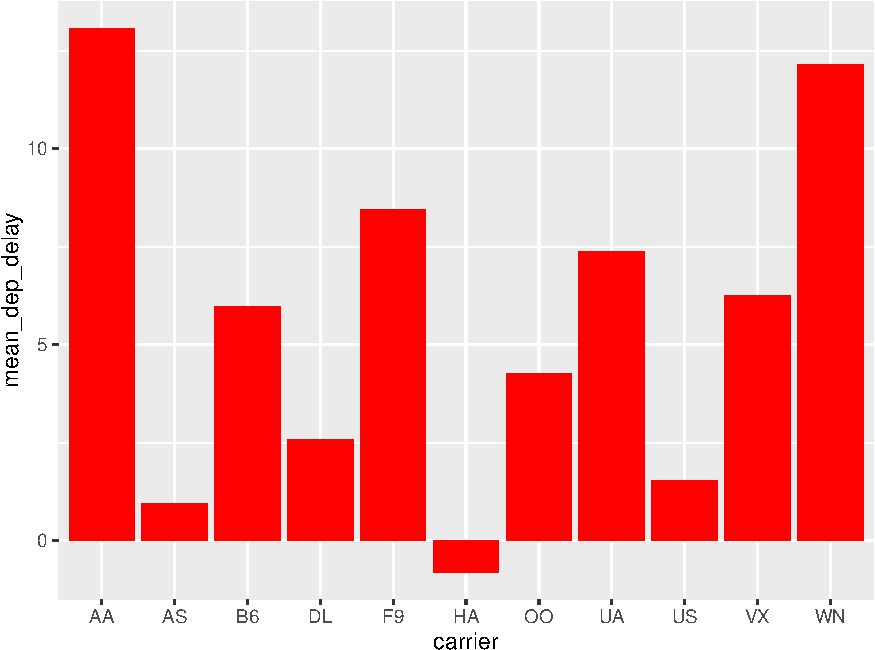
\includegraphics{thesis_files/figure-latex/delaysboxplot-1} 
  
  }
  
  \caption[Mean Delays by Airline]{Mean Delays by Airline}\label{fig:delaysboxplot}
  \end{figure}
  
  Here is a reference to this image: Figure \ref{fig:delaysboxplot}.
  
  A table linking these carrier codes to airline names is available at
  \url{https://github.com/ismayc/pnwflights14/blob/master/data/airlines.csv}.
  
  \clearpage
  
  Next, we will explore the use of the \texttt{out.extra} chunk option,
  which can be used to shrink or expand an image loaded from a file by
  specifying \texttt{"scale=\ "}. Here we use the mathematical graph
  stored in the ``subdivision.pdf'' file.
  
  \begin{figure}
  
  {\centering 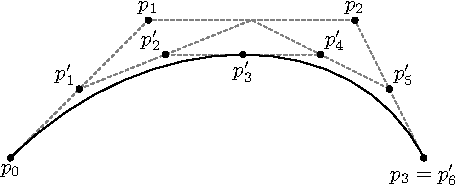
\includegraphics[scale=0.75]{figure/subdivision} 
  
  }
  
  \caption[Subdiv]{Subdiv. graph}\label{fig:subd}
  \end{figure}
  
  Here is a reference to this image: Figure \ref{fig:subd}. Note that
  \texttt{echo=FALSE} is specified so that the \textbf{R} code is hidden
  in the document.
  
  \textbf{More Figure Stuff}
  
  Lastly, we will explore how to rotate and enlarge figures using the
  \texttt{out.extra} chunk option. (Currently this only works in the PDF
  version of the book.)
  
  \begin{figure}
  
  {\centering 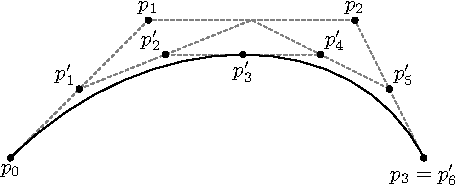
\includegraphics[angle=180, scale=1.1]{figure/subdivision} 
  
  }
  
  \caption[A Larger Figure, Flipped Upside Down]{A Larger Figure, Flipped Upside Down}\label{fig:subd2}
  \end{figure}
  
  As another example, here is a reference: Figure \ref{fig:subd2}.
  
  \section{Footnotes and Endnotes}\label{footnotes-and-endnotes}
  
  You might want to footnote something.\footnote{footnote text} The
  footnote will be in a smaller font and placed appropriately. Endnotes
  work in much the same way. More information can be found about both on
  the CUS site or feel free to reach out to
  \href{mailto:data@reed.edu}{\nolinkurl{data@reed.edu}}.
  
  \section{Bibliographies}\label{bibliographies}
  
  Of course you will need to cite things, and you will probably accumulate
  an armful of sources. There are a variety of tools available for
  creating a bibliography database (stored with the .bib extension). In
  addition to BibTeX suggested below, you may want to consider using the
  free and easy-to-use tool called Zotero. The Reed librarians have
  created Zotero documentation at
  \url{http://libguides.reed.edu/citation/zotero}. In addition, a tutorial
  is available from Middlebury College at
  \url{http://sites.middlebury.edu/zoteromiddlebury/}.
  
  \emph{R Markdown} uses \emph{pandoc} (\url{http://pandoc.org/}) to build
  its bibliographies. One nice caveat of this is that you won't have to do
  a second compile to load in references as standard LaTeX requires. To
  cite references in your thesis (after creating your bibliography
  database), place the reference name inside square brackets and precede
  it by the ``at'' symbol. For example, here's a reference to a book about
  worrying: (Molina \& Borkovec, 1994). This \texttt{Molina1994} entry
  appears in a file called \texttt{thesis.bib} in the \texttt{bib} folder.
  This bibliography database file was created by a program called BibTeX.
  You can call this file something else if you like (look at the YAML
  header in the main .Rmd file) and, by default, is to placed in the
  \texttt{bib} folder.
  
  For more information about BibTeX and bibliographies, see our CUS site
  (\url{http://web.reed.edu/cis/help/latex/index.html})\footnote{Reed~College
    (2007)}. There are three pages on this topic: \emph{bibtex} (which
  talks about using BibTeX, at
  \url{http://web.reed.edu/cis/help/latex/bibtex.html}),
  \emph{bibtexstyles} (about how to find and use the bibliography style
  that best suits your needs, at
  \url{http://web.reed.edu/cis/help/latex/bibtexstyles.html}) and
  \emph{bibman} (which covers how to make and maintain a bibliography by
  hand, without BibTeX, at
  \url{http://web.reed.edu/cis/help/latex/bibman.html}). The last page
  will not be useful unless you have only a few sources.
  
  If you look at the YAML header at the top of the main .Rmd file you can
  see that we can specify the style of the bibliography by referencing the
  appropriate csl file. You can download a variety of different style
  files at \url{https://www.zotero.org/styles}. Make sure to download the
  file into the csl folder.
  
  \textbf{Tips for Bibliographies}
  
  \begin{itemize}
  \tightlist
  \item
    Like with thesis formatting, the sooner you start compiling your
    bibliography for something as large as thesis, the better. Typing in
    source after source is mind-numbing enough; do you really want to do
    it for hours on end in late April? Think of it as procrastination.
  \item
    The cite key (a citation's label) needs to be unique from the other
    entries.
  \item
    When you have more than one author or editor, you need to separate
    each author's name by the word ``and'' e.g.
    \texttt{Author\ =\ \{Noble,\ Sam\ and\ Youngberg,\ Jessica\},}.
  \item
    Bibliographies made using BibTeX (whether manually or using a manager)
    accept LaTeX markup, so you can italicize and add symbols as
    necessary.
  \item
    To force capitalization in an article title or where all lowercase is
    generally used, bracket the capital letter in curly braces.
  \item
    You can add a Reed Thesis citation\footnote{Noble (2002)} option. The
    best way to do this is to use the phdthesis type of citation, and use
    the optional ``type'' field to enter ``Reed thesis'' or
    ``Undergraduate thesis.''
  \end{itemize}
  
  \section{Anything else?}\label{anything-else}
  
  If you'd like to see examples of other things in this template, please
  contact the Data @ Reed team (email
  \href{mailto:data@reed.edu}{\nolinkurl{data@reed.edu}}) with your
  suggestions. We love to see people using \emph{R Markdown} for their
  theses, and are happy to help.
  
  \chapter*{Conclusion}\label{conclusion}
  \addcontentsline{toc}{chapter}{Conclusion}
  
  \setcounter{chapter}{4} \setcounter{section}{0}
  
  If we don't want Conclusion to have a chapter number next to it, we can
  add the \texttt{\{.unnumbered\}} attribute. This has an unintended
  consequence of the sections being labeled as 3.6 for example though
  instead of 4.1. The \LaTeX~commands immediately following the Conclusion
  declaration get things back on track.
  
  \textbf{More info}
  
  And here's some other random info: the first paragraph after a chapter
  title or section head \emph{shouldn't be} indented, because indents are
  to tell the reader that you're starting a new paragraph. Since that's
  obvious after a chapter or section title, proper typesetting doesn't add
  an indent there.
  
  \appendix
  
  \chapter{The First Appendix}\label{the-first-appendix}
  
  This first appendix includes all of the R chunks of code that were
  hidden throughout the document (using the \texttt{include\ =\ FALSE}
  chunk tag) to help with readibility and/or setup.
  
  \textbf{In the main Rmd file}
  
  \begin{Shaded}
  \begin{Highlighting}[]
  \CommentTok{# This chunk ensures that the thesisdown package is}
  \CommentTok{# installed and loaded. This thesisdown package includes}
  \CommentTok{# the template files for the thesis.}
  \NormalTok{if(!}\KeywordTok{require}\NormalTok{(devtools))}
    \KeywordTok{install.packages}\NormalTok{(}\StringTok{"devtools"}\NormalTok{, }\DataTypeTok{repos =} \StringTok{"http://cran.rstudio.com"}\NormalTok{)}
  \NormalTok{if(!}\KeywordTok{require}\NormalTok{(thesisdown))}
    \NormalTok{devtools::}\KeywordTok{install_github}\NormalTok{(}\StringTok{"ismayc/thesisdown"}\NormalTok{)}
  \KeywordTok{library}\NormalTok{(thesisdown)}
  \end{Highlighting}
  \end{Shaded}
  
  \textbf{In Chapter \ref{ref-labels}:}
  
  \begin{Shaded}
  \begin{Highlighting}[]
  \CommentTok{# This chunk ensures that the thesisdown package is}
  \CommentTok{# installed and loaded. This thesisdown package includes}
  \CommentTok{# the template files for the thesis and also two functions}
  \CommentTok{# used for labeling and referencing}
  \NormalTok{if(!}\KeywordTok{require}\NormalTok{(devtools))}
    \KeywordTok{install.packages}\NormalTok{(}\StringTok{"devtools"}\NormalTok{, }\DataTypeTok{repos =} \StringTok{"http://cran.rstudio.com"}\NormalTok{)}
  \NormalTok{if(!}\KeywordTok{require}\NormalTok{(dplyr))}
      \KeywordTok{install.packages}\NormalTok{(}\StringTok{"dplyr"}\NormalTok{, }\DataTypeTok{repos =} \StringTok{"http://cran.rstudio.com"}\NormalTok{)}
  \NormalTok{if(!}\KeywordTok{require}\NormalTok{(ggplot2))}
      \KeywordTok{install.packages}\NormalTok{(}\StringTok{"ggplot2"}\NormalTok{, }\DataTypeTok{repos =} \StringTok{"http://cran.rstudio.com"}\NormalTok{)}
  \NormalTok{if(!}\KeywordTok{require}\NormalTok{(ggplot2))}
      \KeywordTok{install.packages}\NormalTok{(}\StringTok{"bookdown"}\NormalTok{, }\DataTypeTok{repos =} \StringTok{"http://cran.rstudio.com"}\NormalTok{)}
  \NormalTok{if(!}\KeywordTok{require}\NormalTok{(thesisdown))\{}
    \KeywordTok{library}\NormalTok{(devtools)}
    \NormalTok{devtools::}\KeywordTok{install_github}\NormalTok{(}\StringTok{"ismayc/thesisdown"}\NormalTok{)}
    \NormalTok{\}}
  \KeywordTok{library}\NormalTok{(thesisdown)}
  \NormalTok{flights <-}\StringTok{ }\KeywordTok{read.csv}\NormalTok{(}\StringTok{"data/flights.csv"}\NormalTok{)}
  \end{Highlighting}
  \end{Shaded}
  
  \chapter{The Second Appendix, for
  Fun}\label{the-second-appendix-for-fun}
  
  \backmatter
  
  \chapter{References}\label{references-1}
  
  \noindent
  
  \setlength{\parindent}{-0.20in} \setlength{\leftskip}{0.20in}
  \setlength{\parskip}{8pt}
  
  \hypertarget{refs}{}
  \hypertarget{ref-angel2000}{}
  Angel, E. (2000). \emph{Interactive computer graphics : A top-down
  approach with openGL}. Boston, MA: Addison Wesley Longman.
  
  \hypertarget{ref-angel2001}{}
  Angel, E. (2001a). \emph{Batch-file computer graphics : A bottom-up
  approach with quickTime}. Boston, MA: Wesley Addison Longman.
  
  \hypertarget{ref-angel2002a}{}
  Angel, E. (2001b). \emph{Test second book by angel}. Boston, MA: Wesley
  Addison Longman.
  
  \hypertarget{ref-Molina1994}{}
  Molina, S. T., \& Borkovec, T. D. (1994). The Penn State worry
  questionnaire: Psychometric properties and associated characteristics.
  In G. C. L. Davey \& F. Tallis (Eds.), \emph{Worrying: Perspectives on
  theory, assessment and treatment} (pp. 265--283). New York: Wiley.
  
  \hypertarget{ref-noble2002}{}
  Noble, S. G. (2002). \emph{Turning images into simple line-art}
  (Undergraduate thesis). Reed College.
  
  \hypertarget{ref-reedweb2007}{}
  Reed~College. (2007, March). LaTeX your document. Retrieved from
  \url{http://web.reed.edu/cis/help/LaTeX/index.html}


  % Index?

\end{document}

